%!TEX program = xelatex
\documentclass[bachelor]{seuthesis} % 本科
% \documentclass[master]{seuthesis} % 硕士
% \documentclass[doctor]{seuthesis} % 博士
% \documentclass[engineering]{seuthesis} % 工程硕士
\usepackage{CJK,CJKnumb}
\usepackage{hyperref}


% 导言区
\begin{document}
\categorynumber{000} 	% 分类采用《中国图书资料分类法》
\UDC{000}            	%《国际十进分类法UDC》的类号2
\secretlevel{公开}    	% 学位论文密级分为"公开"、"内部"、"秘密"和"机密"四种
\studentid{09013119}   	% 学号要完整,前面的零不能省略。

\title{基于多知识库的表格实体链接系统}{}{Thesis Title}{subtitle}
\author{严晟嘉}{Shengjia Yan}
\advisor{李慧颖}{教授}{Huiying Li}{Prof.}
\coadvisor{漆桂林}{教授}{Guilin Qi}{Prof.}

% \degree{工学硕士} % 详细学位名称
\major[12em]{计算机科学与技术}
\defenddate{答辩日期}
\authorizedate{学位授予日期}
\department{计算机科学与工程}{Computer Science \& Engineering}
\duration{2017.02.20 — 2017.05.22}
\address{东南大学九龙湖校区}
\thanks{}
\maketitle

% 中文摘要
\begin{abstract}{实体链接,Web表格,多知识库}
在当今的万维网上包含着超大规模的蕴含丰富价值的关系型数据,而这些关系型数据大多以 HTML 表格 (也就是 Web 表格) 的形式呈现。
抽取 Web 表格中的语义来制造机器可以理解的知识如今已经成为了一个热门的研究领域。
从 Web 表格中抽取出丰富且高质量的语义信息是一个充满挑战和价值的任务,其中关键一步就是实体链接 (Entity Linking),其目的在于建立表格中的字符串指称 (Mention) 到知识库中的相应实体 (Entity) 的链接。\par

目前大部分的实体链接都是使用单个特定的跨领域知识库来作为实体数据的来源。但由于单个知识库中的实体数量有限且对实体的覆盖范围不广,从而导致单知识库实体链接中实体缺失和链接错误的问题常有发生。
在本文中,我会介绍我的本科毕业设计``基于多知识库的表格实体链接系统''的设计思路和具体实现,这个系统中包含了2种表格实体链接的新方法。与先前的工作不同的是,我的方法使用多知识库而不是单知识库作为实体数据的来源,来提升表格实体链接的质量。\par

方法一是一个``两步走''的方法,我首先将一个基于通用的概率图模型的随机游走算法应用于单知识库的表格实体链接,然后使用多知识库间已有的和新学习到的``sameAs''关系来提升前一步中实体链接结果的质量。
方法二融合了方法一中的两步,我修改了方法一中概率图模型中的节点定义,直接将多知识库间已有的和新学习到的``sameAs''关系融合进了概率图模型,从而实现了一步到位的效果。\par

本文中的所有实验都是在基于 Zhishi.me 人工标注的 Web 表格上进行的,Zhishi.me 涵盖了三个最大的中文百科知识库:百度百科,互动百科和中文维基百科。实验结果表明我的方法在一些评估指标上胜过当今最好的表格实体链接方法。
除此之外,系统在实体消岐时引入了更多的有效的特征,还增加了一些有意义的功能,比如实体链接和``sameAs''关系的迭代学习,在表格实体链接完成之后进行表格的关系抽取。
\end{abstract}

% 英文摘要
\begin{englishabstract}{Entity Linking, Web Tables, Multiple Linked Knowledge Bases}
The World-Wide Web contains a huge scale of valuable relational data, which are embedded in HTML tables (i.e. Web tables). It's a challenging and valuable task that extracting abundant and high-quality semantics of Web tables is. A key step in extracting the semantics of Web tables is Entity Linking (EL), which aims to map the string mentions in table cells to their referent entities in a Knowledge Base (KB).\par

At present most entity linking researches use single cross-domain KBs as source of entities. However, the quantity of entities and the coverage in a single KB is limited. Thus, the issues of entity absence and linking error often appear in the process of EL in a single KB. In this paper, I will introduce the design ideas and concrete implementations of my undergraduate graduate project ``Entity Linking System in Web Tables with Multiple Linked Knowledge Bases'', which includes two new approaches for EL in Web tables. Different from previous work, the proposed approaches replace a single KB with multiple linked KBs as the sources of entities to improve the quality of EL.

Approach One is a two-step method. I first apply a random walk algorithm based on a general probabilistic graphical model to EL in Web tables with each single KB. Then, I leverage the existing and newly learned ``sameAs'' relations between the entities from different KBs to help improve the results of EL in the first step. Approach Two merges two steps from Approach One. I modify node definitions in the probabilistic graphical model in Approach One and directly add the ``sameAs'' relations between the entities from different KBs into the model.\par

All experiments are conducted on the sampled Web tables with Zhishi.me, which consists of three biggest linked Chinese encyclopedic KBs: Baidubaike, Hudongbaike and Zhwiki. The experimental results show that my approaches outperform the state-of-the-art table's EL methods in different evaluation metrics. Besides, the system adds some meaningful functions, such as iterative learning between EL and ``sameAs'' relations and table's relation extraction after EL in Web tables is accomplished.
\end{englishabstract}

% 目录
\tableofcontents

% 术语表
% \begin{terminology}

\begin{table}[h]
%\Large
\begin{tabular}{|>{\LARGE}m{0.2\textwidth}<{\centering}|m{0.8\textwidth}|}
\hline
\normalsize \hspace*{\stretch{1}}术语\hspace*{\stretch{1}} & \hspace*{\stretch{1}}含义\hspace*{\stretch{1}} \\ 
\hline
a & 如同汉字起源于象形,拉丁字母表中的每个字母一开始都是描摹某种动物或物体形状的图画\\
\hline
b & 和A一样,字母B也可以追溯到古代腓尼基。在腓尼基字母表中B叫beth,代表房屋,在希伯来语中B也叫beth,也含房屋之意。\\
\hline
c& 字母C在腓尼基人的文字中叫gimel,代表骆驼。它在字母表中的排列顺序和希腊字母Γ(gamma)相同,实际上其字形是从后者演变而来的。C在罗马数字中表示100。\\
\hline
d&D在古时是描摹拱门或门的形状而成的象形符号,在古代腓尼基语和希伯来语中叫做daleth,是“门”的意思,相当于希腊字母Δ(delta)。\\
\hline
\end{tabular}
%\caption{my table}
\end{table}

\end{terminology}

% 开始正文
\begin{Main}

\chapter{绪论}

\section{研究动机}
如今 Web 上的内容每天都在以指数级的速度增长\cite{limaye2010annotating},这也使得 Web 近年来成为世界上最大的数据集散地之一。
据估计 Web 上有超过141亿张表格,其中1.54亿张表格包含关系型数据并且仅 Wikipedia 就是大约160万关系型表格的来源。
可见Web 表格,换句话说是 Web 上的 HTML 表格,是关系型数据的一个重要来源和信息抽取 (Information Extraction) 系统的一个重要输入。
与普通文本不同,单张关系型表格就包含一系列高质量的关系实体并且在表格的表头中包含与实体相关的元数据。
Web 上包含关系型数据的表格中蕴含的巨大财富和价值使得表格的语义解释 (Semantic Interpretation),也就是将 Web 表格转换成机器能够理解的知识这一任务成为热门的研究领域。\par

另一方面,诸如维基百科等知识共享社区的蓬勃发展和信息抽取技术的进步已经促成了大规模机器可读知识库的自动化建设。
目前世界上已经出现了上百个领域不同、规模不一的知识库 (Knowledge Base) 并且它们的规模每天都在飞速增长。知识库中包含着整个世界的实体,实体的语义类别及其相互关系的丰富信息。
这样典型的例子包括 YAGO\cite{suchanek2007yago},DBpedia\cite{auer2007dbpedia} 和 Freebase\cite{bollacker2008freebase}。
在中文知识库中较有影响力的就是由上海交通大学和东南大学共同建立的 Zhishi.me\cite{niu2011zhishi}。\par

Web 上虽然蕴含着许多有价值的数据,但更多的却是各种原始并且充斥着噪声的数据,其中有些甚至是错误的。
这些数据大都是以自然语言的形式存在,然而由于自然语言表达的多样性与歧义性,使得它们很难被计算机直接处理或者理解。
面对如此规模庞大而嘈杂的数据,信息过载的现象每天都在发生。
信息过载意味着在找到想要的有用的信息之前,需要处理大量的无用数据,计算机获取有效信息的效率常常受到限制。
为了减轻信息过载带来的负面影响以及处理自然语言的多样性问题和歧义性问题,语义网 (Semantic Web) 的概念应运而生,旨在对现有万维网上的文档进行元数据 (Meta Data) 标注,使计算机能够理解词语和概念以及它们之间的逻辑关系。
将 Web 数据与知识库链接起来是非常有利于标注 Web 上的大规模数据的,并且有助于实现语义网的愿景\cite{berners2001semantic}。
许多为了解释说明 Web 表格内含的语义的研究工作\cite{limaye2010annotating}\cite{hignette2009fuzzy}\cite{mulwad2013semantic}\cite{munoz2014using}\cite{syed2010exploiting}\cite{venetis2011recovering}是将其内容标注成 RDF 三元组。
这种语义标注 (Semantic Annotation) 的关键一步就是实体链接 (Entity Linking),将出现在 Web 表格单元格中的字符串指称 (Mention) 链接到其在给定知识库中对应的参考实体 (Entity)。\par

实体链接技术的发展可以带动许多不同的应用的发展,比如知识库补全,自然语言问答系统和语义搜索系统。
随着社会的发展,新的知识被创造出来并以数据的形式表现在 Web 上。
因此,利用这些新知识扩充现有的知识库显得越发重要。
然而,为了将这些新知识插入到现有知识库中,会不可避免地需要一个系统,来将字符串指称,也就是与已抽取出的知识相关联的指称,链接到知识库中的相应实体。
例如,自然语言问答系统依靠它们支持的知识库来回答用户的问题。
为了回答``苹果公司创始人史蒂夫·乔布斯的诞生日期是哪天''这个问题,该系统应首先利用实体链接技术将查询语句中的``史蒂夫·乔布斯''映射到美国企业家,而不是美国传记电影,
然后从知识库中直接取回名为``史蒂夫·乔布斯''的出生日期。
除此之外,实体链接对数据集成很有帮助,可以将不同页面、文档和站点上的实体信息进行集成。
可见,Web 表格上的实体链接技术很有价值并且拥有广阔的应用前景。\par


\section{研究现状}

在本节中,我会回顾一些在 Web 表格上进行语义标注的相关研究工作,它们通常会处理三个任务:实体链接 (Entity Linking),列类型推理 (Column Type Inference) 以及关系抽取 (Relation Extraction)。 
在 Cafarella 等人\cite{cafarella2008webtables}报告说,有超过1.5亿个 Web 表格内嵌有高质量的关系型数据,许多研究人员意识到 Web 表格是许多应用的重要数据来源,比如信息抽取和结构化数据搜索。 
因此,与 Web 表格的语义标注相关的各种研究工作如雨后春笋般涌现出来。\par

Hignette 等人\cite{hignette2009fuzzy}提出了一种聚合的方法,使用给定本体中的词汇来标注 Web 表格中的内容。
它首先标注单元格,然后标注列的类型,最后标注列之间的关系。
与之相似的,Syed 等人\cite{syed2010exploiting}提出了一种管道方法,其首先进行列类型推理,然后将单元格的值链接到给定的知识库中的实体,最后选择列之间合适的关系。
Zhang \cite{zhang2014towards}设计了一个名为 TableMiner 的工具来标注 Web 表格。
TableMiner 只专注于列类型推理和实体链接,并不能从 Web 表格中抽取关系。
之后,Zhang \cite{zhang2014learning}又提出了一些策略来改进 TableMiner。 
Limaye 等人\cite{limaye2010annotating}和 Mulwad 等人\cite{mulwad2013semantic}提出了两种方法,可以分别对 Web 表格上的实体链接,列类型推理和关系抽取任务联合建模。
我的方法和这些研究工作之间的主要区别在于它不依赖任何特定的信息来完成实体链接的任务,例如 Web 表格的表头和标题,知识库中的实体类型和网页中的语义标记等等。\par

还有一些在特定场景下对 Web 表格进行语义标注的研究工作是没有实体链接的步骤的。
在 Venetis 等人\cite{venetis2011recovering}的研究工作中,他们的方法是弱化实体链接的影响,直接进行列类型推理,并且通过大规模的关系数据库 (Relation Databases) 中不同模式的出现频率来确定 Web 表格中的关系,这些关系数据库都是由网页构建的,但通常不对大部分研究人员开放。
此外,Munoz 等人\cite{munoz2014using}提出了一种从维基百科表格中挖掘 RDF 三元组的方法。
在这项研究中,他们能够通过内部链接和文章标题直接识别出维基百科中的实体。\par

跟我的方法最相近的研究工作是 Bhagavatula等人\cite{bhagavatula2015tabel} 和 Shen 等人\cite{shen2012liege}的研究工作。
Shen 等人\cite{shen2012liege}尝试将形如列表 (List-like) 的 Web 表格 (表格有多行但只有一列) 中的字符串指称链接到给定知识库中的实体。
Bhagavatula 等人\cite{bhagavatula2015tabel}提出了 TabEL,一个表格实体链接系统,它使用集体分类技术来对 Web 表格中的所有指称进行联合消岐 (Entity Disambiguation)。
这两个研究工作都不使用任何特定信息来进行实体链接,并且可以应用于任何知识库。
在本文中,为了提高 Web 表格中的实体链接的质量,我专注于在多个相互有链接关系的知识库下的实体链接而不是单个知识库下的实体链接。\par


\section{本文贡献}\label{contribution}

之前的 Web 表格实体链接研究中主要存在两个问题。
1) 许多研究工作\cite{limaye2010annotating}\cite{hignette2009fuzzy}\cite{mulwad2013semantic}\cite{syed2010exploiting}\cite{zhang2014towards}\cite{zhang2014learning}都非常依赖于基于特定信息的特征,
比如 Web 表格的表头 (e.g. ``电影'',``导演''等等。在图~\ref{el} 中表格的第一行中出现),目标知识库中的实体类型以及其他的一些特定信息。
假如我们要处理的 Web 表格中没有这样的表头信息抑或是给定的知识库中没有实体类型的信息,那么很显然前面提及的那些方法的效果会很有限。
2) 现在大部分实体链接的方法\cite{limaye2010annotating}\cite{hignette2009fuzzy}\cite{syed2010exploiting}\cite{zhang2014towards}\cite{zhang2014learning}\cite{shen2012liege}\cite{bhagavatula2015tabel}都只考虑将 Web 表格单元格中的字符串指称链接到单一知识库,但是每个知识库中的实体数量都是有限的,单一知识库无法保证在做 Web 表格上的实体链接的时候对实体有一个很好的覆盖度。
单知识库上的实体链接常常会出现实体缺失的状况。这个问题在这篇论文\cite{pereira2014entity}中的自然语言文本上实体链接的过程中也有体现。\par

为了克服上述问题,在我的毕业设计``基于多知识库的表格实体链接研究''中,我提出了两个新的通用的方法来做基于多知识库的 Web 表格实体链接。
1) 方法一中包含两个步骤。第一步是将一个不依赖于任何特定信息的基于图模型 (Probabilistic Graph Model) 的算法用来做 Web 表格与每个单知识库的实体链接。
然后在第二步中,我提出了三个启发式规则,利用来自不同知识库的实体之间的已存在的和新学习的 ``sameAs'' 关系,以提高第一步的实体链接结果的质量。
第二步不仅可以减少单知识库实体链接产生的错误,还可以提高实体链接结果的覆盖范围。
2) 方法二基于一种融合的思想,尝试用一个统一的图模型来表示 Web 表格中的字符串指称和来自多知识库的实体信息,然后在这个图模型上进行随机游走 (Random Walk),直接得到实体链接的结果。
简单的说,方法二融合了方法一中的两步,将多知识库间的 ``sameAs'' 关系加进了图模型,
同时也舍弃了方法一中的启发式规则,毕竟启发式规则是基于直觉和经验而定,在实际操作中有可能会因为多知识库间 ``sameAs'' 关系的缺失而舍弃一些非常有价值的实体链接结果,方法二规避了这些风险。
在实验中,我将一些 Web 表格样本中的字符串指称与 Zhishi.me\cite{niu2011zhishi} 中的实体进行链接,Zhishi.me 是最大的中文链接开放知识库,如图~\ref{zhishime_link} 所示,其由三个相互链接的中文在线百科知识库组成:中文维基百科\footnote{\url{https://zh.wikipedia.org}},百度百科\footnote{\url{http://baike.baidu.com}}和互动百科\footnote{\url{http://www.baike.com}}。

针对本文中的两个方法,设计了一些对比试验来将它们和目前最先进的实体链接系统 (即 TabEL\cite{bhagavatula2015tabel} 和 LIEGE\cite{shen2012liege}) 进行各方面的比较。
实验结果表明,本文中提出的方法在 MRR(即 Mean Reciprocal Rank\footnote{\url{https://en.wikipedia.org/wiki/Mean_reciprocal_rank}} 平均倒数排名),准确率,召回率和 F1 值等评价指标上都表现得很不错。
实验中用到的表格语料库和算法的实现代码\footnote{\url{https://github.com/yanshengjia/link}}都是公开的,人工标注实体的表格数据同样也对未来的表格实体链接研究者开放。\par

% Fig
\begin{figure}[htbp]
\centering
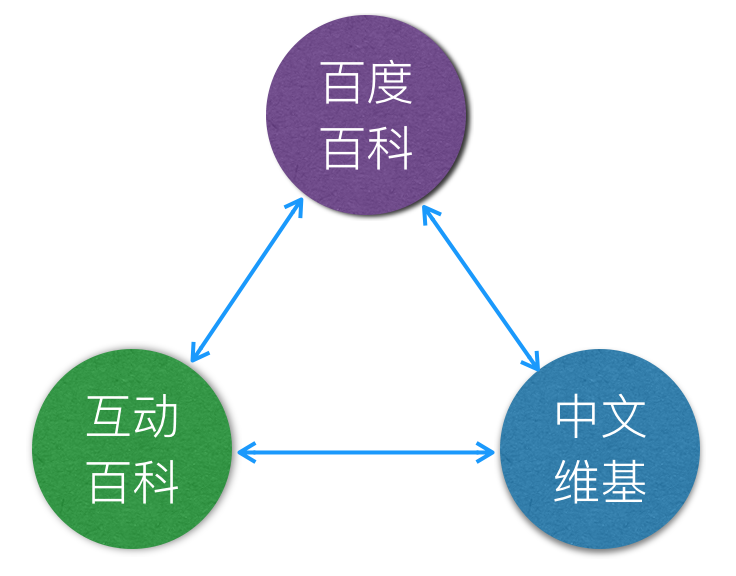
\includegraphics[width=0.4\textwidth]{img/zhishime_link}
\caption{Zhishi.me 由三个相互链接的知识库组成}
\label{zhishime_link}
\end{figure}

总而言之,本文的主要贡献在于:
\begin{enumerate}[1.]
  \item 提出了一个两阶段的基于多知识库的表格实体链接方法 (即方法一),并在实验中体现其比基于单一知识库的实体链接方法的优越性。该方法不依赖表格和知识库中的特定信息,而是建立了一个通用的图模型并使用随机游走算法来进行实体的迭代消岐。
  \item 提出了一个融合的支持多知识库的表格实体链接方法 (即方法二),其融合了方法一中的两步,规避了方法一中的启发式规则带来的风险,整个方法都是在一个统一的图模型上运行,一步到位得得出链接结果。
  \item 设计了一些对比试验,将本文提出的两个方法,TabEL\cite{bhagavatula2015tabel} 和 LIEGE\cite{shen2012liege} 在链接准确率、召回率、F1 值和 MRR 值上进行比较,从而验证本文提出的两个方法的效果。
  \item 在实体消岐时相较于以前的方法使用了很多十分具有价值的特征,比如字符串相似度特征、上下文相似度特征、同义词特征、三元组关系特征、知识库实体的消岐义特征等等。
  \item 添加了一些很有意义的功能,比如``sameAs'' 关系的学习。多知识库间的 ``sameAs'' 关系往往是不完备的,利用实体链接的结果可以与``sameAs''关系进行迭代学习,另外也可以通过监督学习分类器 SVM\cite{tong2001support} 进行``sameAs''关系的学习。
\end{enumerate}

本文的各章节内容是这样分配的:第一章是绪论的,介绍了我的毕设项目的研究动机、相关研究工作以及本文的主要贡献;
第二章从背景知识的角度出发阐述了基于多知识库的实体链接技术的方方面面,包括任务目标、关键挑战以及一般链接流程;
第三章详细介绍了我的毕设研究中提出的两个方法的思想以及相关模型;
第四章从算法具体实现的角度切入,以一个工程师的身份讲述实现细节;
第五章是实验与评估,详述了整个实验流程,将本文中的两个方法与 TabEL\cite{bhagavatula2015tabel} 和 LIEGE\cite{shen2012liege} 在不同评价指标上进行对比并分析;
第六章也就是最后一章总结了全文,并展望了未来工作。













\chapter{基于多知识库的表格实体链接}

\section{任务描述}


\section{关键挑战}



\section{链接流程}



\section{本章小结}
\chapter{系统描述}

在本章中,我会详细描述系统中使用的概率图模型、随机游走算法以及2个方法的细节。
这2个方法是平行的,方法一是一个两阶段的方法,方法二是方法一的改版,其融合了方法一中的两步,这两个方法的输入和输出都是一样的。
输入都是 Web 表格和多知识库的实体数据,输出都是表格的实体链接结果,即表格中的字符串指称最终链接到的知识库中对应的参考实体。
换句话说,这2个方法中的任何一个都可以单独拿出来作为一个表格实体链接系统的核心算法。
我将这2个方法放在同一个系统中是为了可以更好地比较二者的效果差异。
在使用这个系统时,可以任意选择一个方法,然后得到已选择方法计算得到的实体链接结果。
目前实体链接的方法大体上可以分为3类:基于概率统计的方法,基于机器学习的方法和基于图模型的随机游走方法。
系统中的2个方法都是属于基于图模型的随机游走方法。
这类方法的思路与另外2类方法完全不同。
它主要利用字符串指称与实体之间、实体与实体之间的语义相关性来开展实体链接的工作。
它认为在位置上相邻的字符串指称往往具有语义相关性,比如表格中同行或者同列的指称描述的一般是同一个事物。
在我的方法中,会将字符串指称和知识库实体建模成一张概率图 (Probabilistic Graph Model),称之为实体消岐图 (Entity Disambiguation Graph),然后在这张图上运行随机游走 (Random Walk) 算法进行迭代消岐,直到图上实体节点的概率值收敛,最终得到链接结果。


\section{概率图模型}




\section{随机游走}




\section{方法一: 两步走}

方法一包含2个主要的步骤:首选使用各个单知识库进行实体链接,然后运行多知识库间的 ``sameAs'' 关系来优化单知识库的链接结果。

% Fig 3.1
\begin{figure}[htbp]
\centering
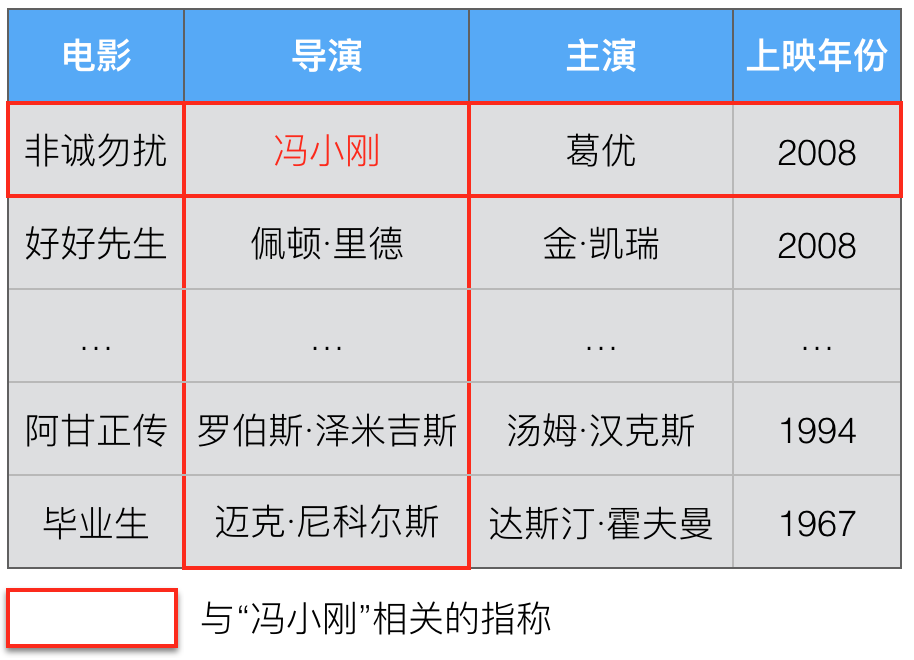
\includegraphics[width=0.6\textwidth]{img/relate}
\caption{一个表格同行同列中的指称具有语义相关性的例子}
\label{relate}
\end{figure}

\subsection{单知识库表格实体链接}

\noindent\textbf{指称识别}\newline
任何实体链接系统的第一步是识别出潜在的字符串指称,它们能够被链接到知识库中的参考实体。
给定来自输入的表格中每个单元格的文本内容,$t_q$,系统将 $t_q$ 中满足一定条件的最长的短语 $s$ 识别为潜在的指称。
这个条件就是对于某些实体 $e$,字符串 $s$ 能链接到该实体的概率 $P(e|s)$ 非零。
如果 $s$ 的长度小于 $t_q$ 的长度,系统会在 $s$ 之后发现长度最长的短语,并以此类推。
例如,对于一个单元格的文本 ``习近平 \& 彭丽媛'',系统会识别出到两个潜在的指称:一个是``习近平'',另一个是``彭丽媛''。\newline


\noindent\textbf{候选实体生成}\newline
对于表格单元格中的每个字符串指称,首先需要从给定的海量的知识库实体中找出一些可能成为该指称参考实体的实体,来缩小实体链接的范围。
这样的实体称为字符串指称的候选实体。这样的过程叫做生成候选实体。
在系统中,我讲每个指称分割到单词级别,所以每个指称能被表示为一个单词集合。
如果给定知识库中的一个实体 $e$ 或者 $s$ 在 BabelNet\cite{navigli2010babelnet} (一个全网域多语种同义词辞典) 中的一个同义词包含某个指称 $m$ 的分割单词集合中的至少一个单词,那么实体 $e$ 就被认为是指称 $m$ 的一个候选参考实体。
举个例子,字符串指称``苹果''有这样的一些候选实体:``苹果'',``苹果派'',``苹果 [水果]'',``苹果 [智能手机品牌]''。
候选实体生成的结果就是每个指称都可能指向一个候选实体集合。
在实际操作过程中,除了指称与实体的包含关系,我还考虑了二者之间的字符串相似度 (计算公式在后面会提到),设置了一个字符串相似度的阈值。
一般来说,与指称的字符串相似度很低的实体,很有可能表示的是跟指称完全不同的事物,即便它们有包含关系。
所以如果实体 $e$ 和指称 $m$ 的字符串相似度低于阈值,即使 $e$ 包含 $m$,也不将该实体 $e$ 添加进 $m$ 的候选实体集合。
比如,对于指称``苹果'',在知识库中有这样的一个实体``苹果红蜘蛛'',显然二者不可能相链接,虽然这个实体里包含了``苹果''二字,但是由于二者的字符串相似度太低,这样的实体就被剔除了。\newline

\noindent\textbf{实体消岐}\newline







\subsection{多知识库优化实体链接}

\begin{figure}[htbp]
\centering
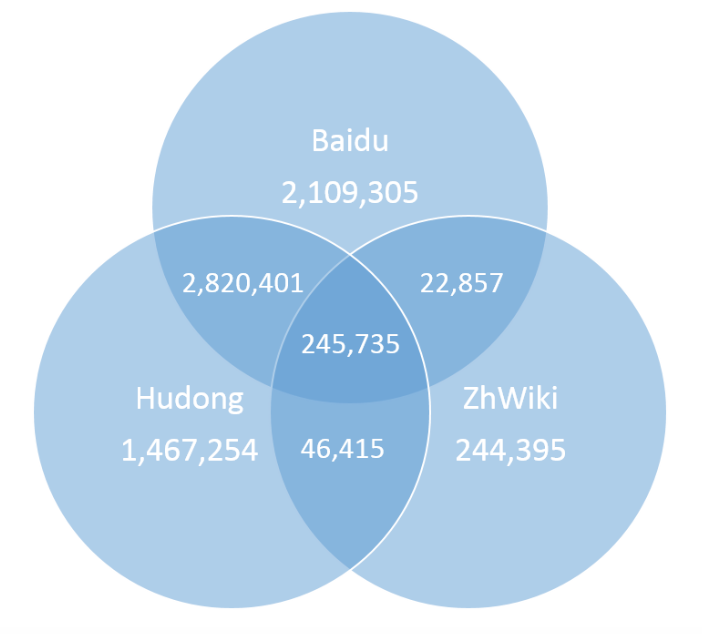
\includegraphics[width=0.4\textwidth]{img/zhishime_data}
\caption{Zhishi.me 数据统计}
\label{zhishime_data}
\end{figure}




\section{方法二: 融合}

\section{EL 与 sameAs 迭代学习}

\section{本章小结}

\chapter{系统实现}

\section{表格语料库}

\section{知识库实体}

\section{人工标注指称来源}

\section{本章小结}

\chapter{实验与评估}
在本章中,我使用 Zhishi.me 中的三个相互链接的知识库 (中文维基百科,百度百科和互动百科) 评估了系统中的方法。
整个评估过程基于人工标注的 Web 表格。
并且将系统中的方法与两个先进的 Web 表格实体链接系统以及我的方法的两个退化版本 (Degenerate Version) 进行比较。

\section{评价标准}
我在每张人工标注过的 Web 表格上使用系统中的方法进行实体链接并用设计好的对比实验进行对比。
在实验中,使用了四个指标 (Metric) 来衡量链接结果的质量。
它们分别是准确率 (Precision),召回率 (Recall),F1值 (F1-score) 和 平均倒数排名 (Mean Reciprocal Rank\cite{craswell2009mean}, MRR)。
这些评价指标普遍用于文本的实体链接任务\cite{bhagavatula2015tabel}。
F1值是准确率和召回率的调和平均数。
平均倒数排名 (MRR) 用来评估指称的候选实体排名列表的质量。
对于一个指称 $m$,实体链接的倒数排名 (Reciprocal Rank) 是 $m$ 的正确参考实体在候选排名列表中的排名的倒数。
比如,$m$ 的正确参考实体在由实体链接算法生成的候选实体排名列表中排在第二位,则倒数排名为 $\frac{1}{2}$。


\section{几种方法的比较}
我对以下方法进行了对比试验。

\begin{itemize}
  \item[$\bullet$] $TabEL$: TabEL\cite{bhagavatula2015tabel} 是目前 Web 表格实体链接领域先进的系统,它使用一种使用了许多通用特征的集体分类技术来对一个给定 Web 表格中的所有指称进行联合消岐。除此之外,任何知识库都可以被应用于 TabEL 来执行 Web 表格上的实体链接任务。
  \item[$\bullet$] $LIEGE$: LIEGE\cite{shen2012liege} 是一个通用方法,用于将形如列表 (List-like) 的 Web 表格 (多行一列) 中的字符串指称链接到给定知识库中的参考实体。它提出了一种使用了三个特征的迭代置换算法来执行 Web 列表中的实体链接。这个方法同样可以用于任何知识库上的 Web 表格实体链接。
  \item[$\bullet$] $single$: 是 $approach1$ 的一个退化版本。它只使用了方法一中单知识库实体链接的算法,并没有运用三条启发式规则和``sameAs''关系来执行多知识库对实体链接结果的优化算法。
  \item[$\bullet$] $multiple$: 也是 $approach1$ 的一个退化版本。在执行完单知识库实体链接算法后,它仅使用了已存在的``sameAs''关系 (不包括新学习到的``sameAs''关系) 来提升实体链接结果质量。
  \item[$\bullet$] $approach1$: 即为~\ref{approach1} 节描述的方法一。它分为两步,先用每个单知识库进行实体链接,然后用多知识库间的``sameAs''关系进行链接结果的优化。它采用了一种基于图的随机游走算法来实现一个表格中所有指称的联合消岐。同样,它也是一个通用算法,任何拥有丰富 RDF 三元组格式数据的知识库都可以作为该方法的输入。
  \item[$\bullet$] $approach2$: 即为~\ref{approach2} 节描述的方法二。它融合了方法一中的两步,使用了一个统一的图模型来表示一个给定表格的所有指称和候选实体以及多知识库间的``sameAs''关系。它也是一个适用于任何知识库的多知识库实体链接算法。
\end{itemize}

% Table
\begin{table}[htbp]
\centering
\caption{由三个单知识库衡量的总体实体链接结果}
\label{result}
\begin{tabular}{|c|c|c|c|c|c|}
\hline
Knowledge Base & Approach & Precision & Recall & F1-score & MRR \\
\hline
\multirow{6}{*}{Chinese Wikipedia} & TabEL & 0.823 & 0.809 & 0.816 & 0.858 \\
\cline{2-6} & LIEGE & 0.778 & 0.747 & 0.762 & 0.813 \\
\cline{2-6} & single & 0.830 & 0.797 & 0.813 & 0.860 \\
\cline{2-6} & multiple & 0.861 & 0.821 & 0.841 & 0.881 \\
\cline{2-6} & approach1 & \textbf{0.873} & \textbf{0.828} & \textbf{0.850} & \textbf{0.887} \\
\cline{2-6} & approach2 & \textbf{0.856} & \textbf{0.830} & \textbf{0.843} & \textbf{0.814} \\
\hline
\multirow{6}{*}{Baidu Baike} & TabEL & 0.659 & 0.628 & 0.643 & 0.707 \\
\cline{2-6} & LIEGE & 0.629 & 0.576 & 0.601 & 0.670 \\
\cline{2-6} & single & 0.696 & 0.652 & 0.673 & 0.725 \\
\cline{2-6} & multiple & 0.758 & 0.705 & 0.731 & 0.746 \\
\cline{2-6} & approach1 & \textbf{0.774} & \textbf{0.727} & \textbf{0.750} & \textbf{0.776} \\
\cline{2-6} & approach2 & \textbf{0.769} & \textbf{0.747} & \textbf{0.758} & \textbf{0.780} \\
\hline
\multirow{6}{*}{Hudong Baike} & TabEL & 0.681 & 0.649 & 0.665 & 0.780 \\
\cline{2-6} & LIEGE & 0.661 & 0.632 & 0.646 & 0.751 \\
\cline{2-6} & single & 0.708 & 0.642 & 0.673 & 0.768 \\
\cline{2-6} & multiple & 0.729 & 0.700 & 0.714 & 0.787 \\
\cline{2-6} & approach1 & \textbf{0.744} & \textbf{0.708} & \textbf{0.726} & \textbf{0.796} \\
\cline{2-6} & approach2 & \textbf{0.731} & \textbf{0.712} & \textbf{0.721} & \textbf{0.788} \\
\hline
\end{tabular}
\end{table}


\section{结果分析}
表格~\ref{result} 给出了系统中两个实体链接方法的总体结果和由三个单知识库分别衡量的对比实验的结果,从中我可以发现:
\begin{itemize}
  \item[$\bullet$] 方法一中的单知识库实体链接方法,也就是 $single$,其效果能够与当前非常先进的实体链接系统 TabEL 相媲美,并且胜过 LIEGE。这反应了我在系统中提出的方法的有效性。
  \item[$\bullet$] $multiple$ 方法在准确率、召回率、F1值和 MRR 上总是比 $single$ 方法更好。这表明方法一中提出的启发式规则在提升单知识库实体链接结果上是非常有价值的。
  \item[$\bullet$] 系统中的方法一,也就是 $approach1$,在准确率这个指标上比其他所有对比方法都高,这证实了方法一在多知识库 Web 表格实体链接上的优越性。与 $multiple$ 方法相比,方法一具有更好的表现,这体现了新学习到的``sameAs''关系对于解决用不同知识库进行单知识库实体链接 ($single$) 导致的链接冲突问题是很有帮助的。
  \item[$\bullet$] 系统中的方法二,也就是 $approach2$,在准确率这个指标上仅次于方法一,这体现出方法二也是非常有效的。而且与 $approach1$ 相比,$approach2$ 在召回率这个指标上表现更佳,这说明方法一中的启发式规则由于不稳定性导致没有覆盖到一些正确的参考实体,而方法二弥补了这一点。
\end{itemize}
另外,我用整个 Zhishi.me 来衡量的方法一 ($approach1$) 的实体链接结果,并计算了准确率、召回率、F1值。
准确率是0.831,召回率是\textbf{0.903},F1值为0.866。
可以发现召回率有了显著的提升,这表明多知识库的表格实体链接方法的确能够保证一个很好的实体覆盖度。


\section{本章小结}
本章首先介绍了对比试验的评价指标:准确率、召回率、F1值和 MRR。这些都是常见的实体链接算法的评价指标。
然后描述了我设计的六组对比试验,并以表格的形式给出了对比结果。
最后对实体链接的结果进行了对比分析,试验结果表明系统中的多知识库表格实体链接方法的有效性并且相对于单知识库实体链接能够有一个更好的实体覆盖度。
\chapter{总结与展望}

\section{工作总结}
在这篇论文中,我提出了两个新的基于多知识库的表格实体链接方法。
两个方法的核心都是基于图的随机游走算法。
方法一的第一步是用一个基于图的迭代概率传播算法来进行单知识库实体链接。
在第二步中我提出了三条启发式规则来利用不同知识库实体间的``sameAs''关系来提升第一步的链接结果,同时也解决了多知识库实体链接结果冲突的问题。
方法二中使用了一个统一的图模型,直接将多知识库的实体和实体间的``sameAs''关系融合进实体消岐图,一步到位地计算出实体链接结果。
两个方法都有各自的优缺点。
优点在于二者都不依赖特定的信息 (表格的列头,知识库中的实体类型),
并且都是基于多知识库进行实体链接,弥补了单知识库实体覆盖程度不够的缺点。
方法一的缺点在于其第二步中的启发式规则的不稳定性。
方法二的缺点在于,在构建实体消岐图的时候,很多正确的参考实体由于``sameAs''关系缺失的原因不能和其他等价的实体进入同一个实体组结点,又因为链接的目标是为一个给定的指称选择一个实体组结点作为链接结果,作为这样就导致了最终链接结果会有所遗漏。
我设计并实现了两个方法与 TabEL\cite{bhagavatula2015tabel},LIEGE\cite{shen2012liege} 以及另外两个退化版本的方法的对比实验。
实验结果表明本文中的两个方法在不同的评价标准 (准确率、召回率、F1值和 MRR) 上表现得都非常优秀。
并且这两个多知识库表格实体链接方法都非常有效并且相对于单知识库实体链接有一个更好的实体覆盖度。
值得一提的是,本文中的两个方法都是通用的,可以使用任何单知识库或者相互链接的多知识库进行 Web 表格上的实体链接。


\section{未来展望}
在~\ref{challenge} 节中提到当前实体链接的关键挑战在于缺少基准数据集。
因此对于未来的工作,首要任务是建立更多的其他语言的基准数据集,用于开展基于多知识库的 Web 表格实体链接的新任务。
其次是改进优化本文中提出的方法,比如在计算实体链接影响因子的时候设计更多的特征,原先使用的特征主要反映的是指称与实体之间、实体与实体之间的语义相关度,更多有效特征的加入可以多维度地反映指称与实体之间、实体与实体之间的关系,从而提升链接的质量。
更进一步地,衡量本文中的方法在其他语言上,特别是英语上的效果。
除此之外,我还考虑加上关系抽取的功能。
就像~\ref{task} 节中提到的,关系抽取是表格语义解释的主要任务之一。
根据表格中不同列实体链接的结果,通过两列某一行的关系即可得到表格列之间的关系,最终的结果表示为 RDF 三元组。
然后,我计划把本文中的方法进行封装,做成编程接口,提供 API 或者工具供他人使用,或者将这些接口做成 Web 应用,让他人通过 Web 就能轻松使用我的方法进行实体链接。
最后,我考虑将上述方法拓展成跨语言\cite{zhang2013cross} (Cross-lingual) 的多知识库表格实体链接方法。









\end{Main}
% 结束正文

% 致谢
\begin{Acknowledgement}
感谢……
\end{Acknowledgement}

% 参考文献
\bibliography{seuthesis}

\begin{Appendix}
  \chapter{第一个附录}
  ……
\end{Appendix}

\newpage
\printindex % 索引

% \begin{thebibliography}{99}
% \bibliographystyle{spmpsci}
% \bibliography{seuthesis}

% 作者简历
\begin{Resume}
作者简介
\end{Resume}

\end{document}